\section{Capteurs et actuateurs des footbots}

Comme présenté plus haut, les capteurs et actuateurs des agents déterminent bien évidemment les informations qu'ils sont capables de recuellir et les actions qu'ils peuvent effectuer.

\begin{figure}[htb]
   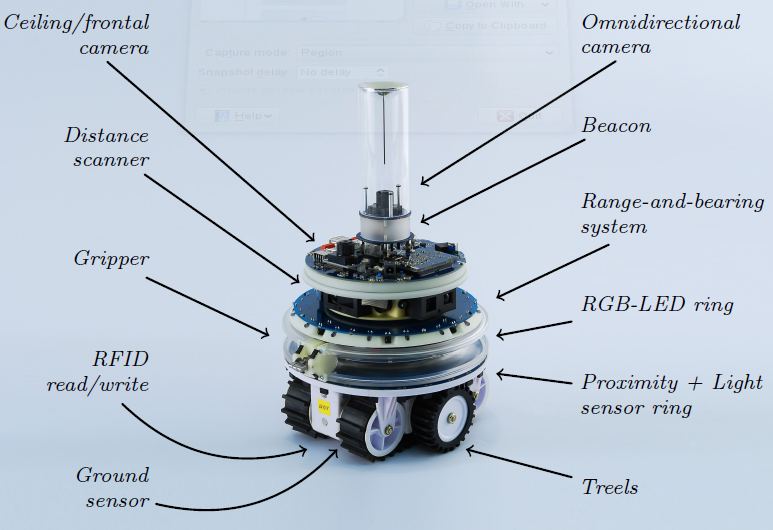
\includegraphics[width=\textwidth]{pics/footbot.png}
      \caption{Les différents senseurs et actuateurs d'un footbot~\cite{argosSite1}}
\end{figure}

Dans le cadre du projet, on considère qu'il suffit que le robot passe sur une <<source>> pour l'exploiter. Les différents capteurs et actuateurs intéressants sont donc les roues, le senseur de proximité et le \emph{distance scanner} pour la partie déplacement, le \emph{ground sensor} pour la partie exploration (car il permet de lire la couleur du sol), et enfin les différentes LED et le système \emph{range and bearing} ainsi que les capteurs associés pour la partie communication.

Comme annoncé dans l'introduction, l'essaim de robots devra être simulé dans ARGoS, un simulateur de robots développé notamment par le département IRIDIA de l'ULB. Ce simulateur a besoin de deux fichiers pour lancer une expérience: un fichier XML qui permet de configurer l'arène et l'expérience en général (moteur physique, capteurs et actuateurs disponibles, \ldots) d'une part, et un fichier dictant le (même) comportement individuel de chaque robot d'autre part. Pour l'instant, les instructions peuvent être écrites soit en C++, soit en Lua.


\section{Choix du langage informatique}

D'une part, les principaux avantages de C++, notamment, sa rapidité exécution et ses nombreuses librairies, ne sont pas primordiaux dans le cadre de ce projet. De plus, il nous est moins familier que Lua qui se rapproche fortement de python tant au niveau de la syntaxe que de l'approche fonctionnelle.

Lua étant un langage de scripting, il est plus adapté aux besoins du groupe car la réalisation du projet passe par de nombreuses petites expérimentations mais ne devrait pas aboutir à un comportement final comportant de très nombreuses lignes de code. En effet, ce type de langage permet de concevoir des prototypes de programmes rapidement.

Enfin sa simplicité et sa lisibilité sont des aspects très importants dans un travail de groupe où chacun doit être capable de comprendre et d'améliorer le comportement en développement \cite{compC++,compLua}.

Au vu des raisons énoncées ci-dessus, Lua a été choisi comme langage de programmation.

\section{Structure d'un comportement en Lua}

Le \emph{template} de code fourni par ARGoS présenté plus bas montre les deux fonctions les plus importantes parmi celles exigées par ARGoS. La fonction \emph{init} qui est éxécutée une fois par chaque footbot au début de l'expérience, et la fonction \emph{step} qui est éxécutée par chaque footbot à chaque pas de la simulation. C'est bien évidemment cette fonction \emph{step} qui représente presqu'entièrement le comportement du robot. Deux types d'évènements peuvent modifier la façon dont cette fonction step s'éxécute: d'une part, les percepts ayant lieu au cours du pas de simulation, et d'autre part un ensemble de variables globales (qui survivent après l'éxécution de la fonction \emph{step} et sont donc accessibles par les instances suivante de cette fonction) qui détermine entièrement l'état du robot lorsque celui-ci entame ce pas de simulation. Enfin, la fonction step peut agir en retour sur ces variables d'état.~\cite{argosSite1}
\begin{lstlisting}[caption=Structure de base d'un comportement en Lua]
--[[ This function is executed every time
     you press the 'execute' button ]]
function init()

end

--[[ This function is executed at each time step
     It must contain the logic of your controller ]]
function step()

end
\end{lstlisting}
